
\documentclass{sig-alternate}

\usepackage{listings}
\usepackage{hyperref}

% Custom colors
\usepackage{color}
\definecolor{deepblue}{rgb}{0,0,0.5}
\definecolor{deepred}{rgb}{0.6,0,0}
\definecolor{deepgreen}{rgb}{0,0.5,0}

\begin{document}
%
% --- Author Metadata here ---
\conferenceinfo{Blocks and Beyond}{'15 Atlanta, Georgia USA}
%\CopyrightYear{2007} % Allows default copyright year (20XX) to be over-ridden - IF NEED BE.
%\crdata{0-12345-67-8/90/01}  % Allows default copyright data (0-89791-88-6/97/05) to be over-ridden - IF NEED BE.
% --- End of Author Metadata ---
% From Interest to Usefulness
\title{BlockPy: From Interest to Usefulness in a Block-based Environment}
\numberofauthors{1}
\author{
	\alignauthor {Austin Cory Bart, Eli Tilevich, Clifford A. Shaffer, Dennis Kafura}\\
	\email{\{acbart, tilevich, shaffer, kafura\}@vt.edu}\\
	\affaddr{Virginia Tech}  \\
}
\date{30 July 1999}

\maketitle
\begin{abstract}
As block-based environments are used for more mature audiences, the environments must mature themselves.
Based on holistic theories of academic motivation, this means making the environment present itself as both Interesting \textit{and} Useful, without sacricing pedagogical power and scaffolding.
We present Data Science as a potential context that satisfies all of these constraints, and describe our new block-based programming environment for education that supports Data Science from day one: BlockPy, available at \url{http://think.cs.vt.edu/blockpy/}.
Blockpy features a number of powerful, authentic features meant to promote transfer for students as they progress.
This includes Mutual Language Translation and interactive feedback, but also powerful tools for getting real-world data and visualizing it.
As we have developed the tool, we have identified a number of major research questions that should be answered in order to determine the validity of our hypothesis and the potential of our approach: in particular, how can this environment and context support educators and diverse learners as they progress into conventional environments.
\end{abstract}

% A category with the (minimum) three required fields
\category{K.3.2}{Computer and Information Science Education}{Computer Science Education}

\terms{Design, Human Factors, Reliability, Experimentation}

\keywords{Blockly, Kennel, Interest, Usefulness} % NOT required for Proceedings


\section{Problem}

How do we bring introductory computing to mature, domain-identified undergraduates, who have concerns for both their own self-efficacy and for the value in learning computing?
Many universities are now defining core credit hours in subjects such as ``Computational Thinking'', introductory computer science classes meant for solving interdisciplinary problems using some degree of programming.
This means that universities now have students of every different discipline and background taking a programming course.
Students with a clearly domain-identified interest (i.e. their actual major) can view introductory computing courses with doubt and suspicion -- what does this course have to offer them, and why should they engage in it?

Our position is that, in order to fully engage all undergraduate students, an introductory programming environment should be both \textit{interesting} and \textit{useful}, while still promoting \textit{success}.
Critically, this means that the environment should enable working with a context that students relate to, enjoy, and helps them solve useful problems.
Further, they should feel that the material that they're learning will help them to transition to more authentic, serious problem-solving of real programming environments.
These changes should not come at the cost of the scaffolding that makes these environments pedagogical valuable, but instead should provide new opportunities for students' learning.

\subsection{Existing Solutions}

Although Block-based environments like Scratch and Snap! have already been successful with high-school students, they may not be suitable for more mature but diverse populations.
In addition to side-stepping syntax headaches, Snap! and Scratch environments make it easier to get working with their motivating educational context, such as game and animation design, robots, or media computation, because they immediately expose the range of actions afforded by the context (e.g., a ``draw a circle'' block for media computation) and support the experiences at a high level (e.g., a drawing canvas embedded within the environment).
These contexts can be very popular with certain classes of students: young male children usually enjoy creating games, for example, so game and animation design is a very compelling hook.
However, many students at the undergraduate level may discreted the usefulness of the environment because the students perceive the environment as a toy rather than a useful tool -- partially because of the puzzle-piece metaphor they utilize, but also because of the contexts that they are providing.

\subsection{A New Solution: Data Science}

We submit \textit{Data Science Exploration} as an educational context that block-based environments should support as a first-class citizen, similar to how Snap! and Scratch support game design.
Data Science for Introductory Computing is a growing movement, with many instructors recognizing the inherent value ~\cite{Anderson, Sullivan:2013}
Data science provides an authentic, useful context for every kind of students, since exploring data-oriented problems is something that almost all fields are beginning to find relevant~\cite{Layman:2007, Social-good}.
Additionally, it is readily possible to find data sources that connect to the world around the student and their past experiences, establishing a sense of personalized interest.
When students inevitably ask, ``What am I going to be using this for?'', it is possible to point to well-defined data problems in their field requiring computation.
This does not mean that we are creating an end-user programming environment for data science, however, but an educational environment that allows students to learn computing principles through the context of data science (similar to how Scratch and Snap! are meant to learn programming, rather than to learn game design).

\begin{figure*}[t]
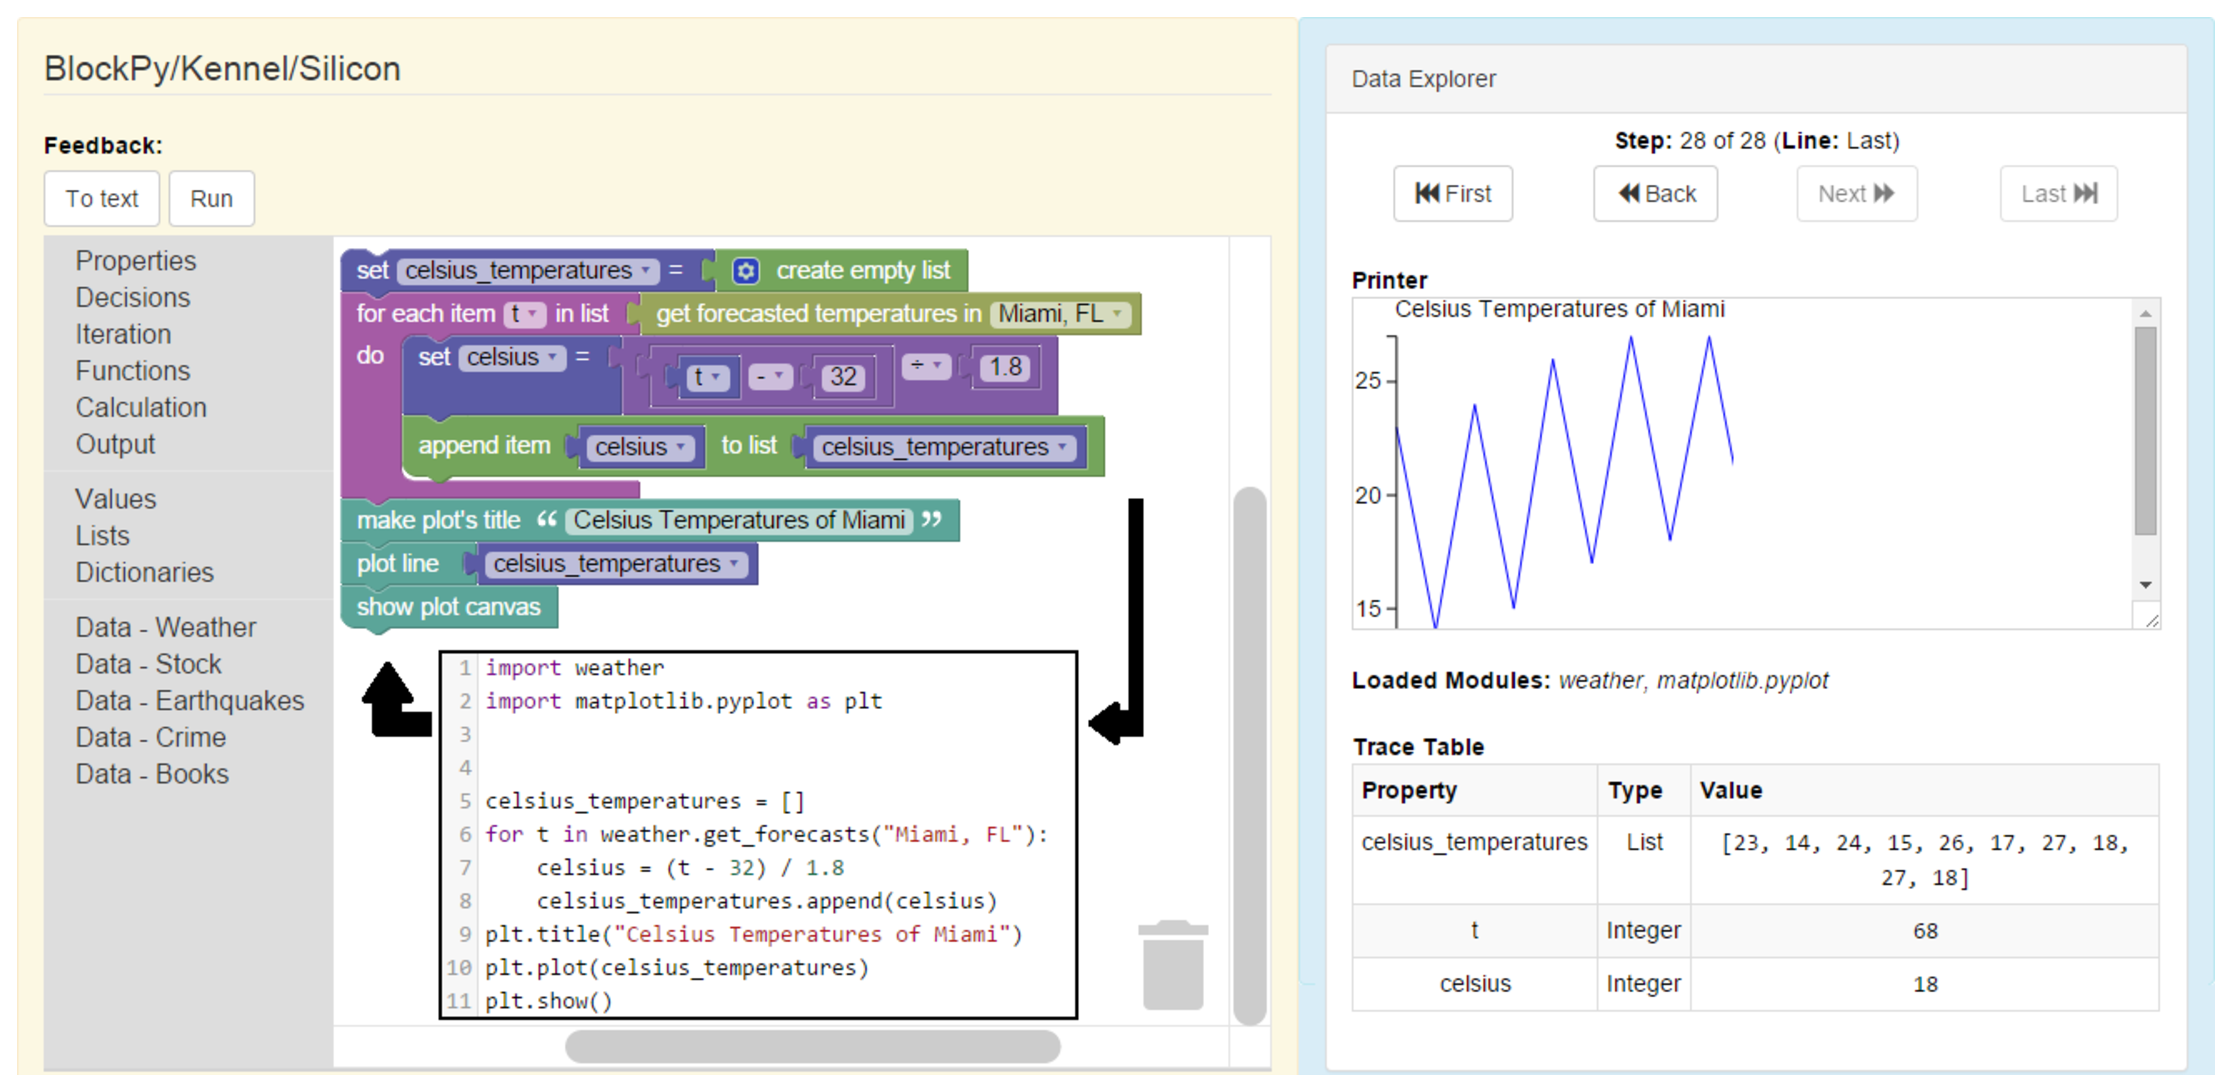
\psfig{file=images/full-kennel.eps, width=\linewidth}
\caption{A complete representation of BlockPy}
\label{fig-blockpy-full}
\end{figure*}

\subsection{Academic Motivation and Blocks}

The prior research on block-based environments in undergraduate settings sheds some light on the limitations of existing environments for those populations.
Mishra conducted a two-week intervention in an introductory course where students worked with Scratch before they began working with Java, reporting positive outcomes in both learning and engagement~\cite{Mishra}.
However, although the sample population was quite large (N=450), the students do not represent the typical body of a university: they were non-CS engineering majors, 88\% male, and ``highest ranked'' in ``mathematics, physics, and chemistry''.
The students did vary greatly on prior programming performance, but their other demographics suggest that they have rather uniform motivational concerns, compared to the general undergraduate population.
In particular, the perception survey revealed that many students cited the game design context afforded by Scratch as a major motivating factor: ``[I am] thrilled to be able to code complex games'' and ``[coding] games helped increase my interest, [...], there was lot of room for experimentation.''
These students valued the game design component because it was interesting to them, but not because they saw it as useful to their careers.
It is unclear how more diverse students would react to this environment.

In our research project, we look at the MUSIC Model of Academic Motivation\cite{jones-description} in order to explain the different ways students become engaged. Specifically, this model differentiates between five different components of motivation: \textbf{eMpowerment}, the amount of control that a student feels that they have over their learning experience; \textbf{Usefulness}, the expectation of the student that the material they are learning will be valuable to their short-term and long-term goals; \textbf{Success}, the student's belief in their own ability to complete their work; \textbf{Interest}, the student's perception of how the assignment appeals to situational or dispositional interests; and \textbf{Caring}, the students perception of their professor's and classmates attitudes toward them.
A student becomes motivated when they perceive one or more of these constructs in their learning experience.
We apply this theory to describe existing game-based programming environments as providing Interest to certain populations, but limited Usefulness.
We suggest that more students (and more typical students) can be better served with a context that supports all five dimensions and, in particular, both general Interest and Usefulness.
To that end, we have created a new block-based environment with this theory in mind.

\newpage

\section{BlockPy}
\url{http://think.cs.vt.edu/blockpy/} 
	
In this section, we concretely describe our work on a new web-based, dual text/block environment:
\textbf{BlockPy}, a beginner-friendly programming environment that scaffolds the learner into a more mature environment while supporting a sense of Usefulness up-front.
Internally, BlockPy uses a modified version of the open-source Blockly library to provide a block editor and a modified version of the open-source Skulpt library to execute Python code client-side.
Figure \ref{fig-blockpy-full} demonstrates the interface: the problem presentation and feedback on the top-left, the dual program representations in the bottom left (via Mutual Language Translation), and the data science dashboard on the right (giving students powerful insight into their programs execution).

\subsection{Data Science as a First-Class Feature}

The code represented in the figure demonstrates the data science API exposed to the student, including blocks and functions to access real-world data sources and to create visualizations.
These data sources include weather forecasts, earthquake reports, and stock feeds.
Data returned from their interface is extremely simple -- usually either primitive (numbers and text) or minimally structured (maps and lists), ensuring that students can begin working with Big Data blocks at the earliest possible points in the course.
In addition to obtaining data, we support the popular MatPlotlib library to provide a set of visualization functions create simple line plots and histograms.
By basing everything around the MatPlotLib API and relying on the Blocks interface for scaffolding, BlockPy seeks to maintain complete compatibility with conventional Python APIs so that all code written is authentic, as opposed to the use of simplified toy APIs in environments like CodeSkulptor.

\subsection{Guided Practice}

BlockPy is not just a code-authoring environment but also a system for guided practice.
Instructors can create problems by writing introductory text and then using an assessment API to define interactive feedback.
Specifically, the instructor can define rules based on students' current code, output, and program state, and gives automatic feedback to the student.
This just-in-time feedback and support is meant to guide students to success.
Of course, the environment also supports free-form coding experiences, as you would find in traditional programming environments; as the students progress through their introductory experience, short-term feedback can decrease and then fade away completely.

\subsection{Transfer to Authenticity}

Although some research is working towards creating end-user block-based environments, we view block-based languages as ``Training Wheels'', meant to be faded away.
Work by Weintrop on the transition from Snap to Python analyzes this transition and offers a number of ways to mediate the transfer through programming tools. 
One of the largest findings is that being able to write inline code inside a Block-based language is extremely helpful to students' learning \cite{Weintrop}.
Another approach we support is Mutual Language Translation, devised by Matsuzawa ~\cite{Matsuzawa}, that creates an isomorphic view of students' code as both text and blocks.
These features are meant to transfer students away from blocks towards text.

\subsection{An Example Scenario}

Consider a lesson for students on Iteration.
The instructor could create a problem asking students to find the average temperature in their local city for this week, using the assessment API to construct rules demanding they use iteration blocks.
Students would begin by dragging in a \texttt{Get Temperatures for [city]} block.
If they attempt to run their code at this point, they will be shown the formula for calculating an average, highlighting the use of iteration (as provided by the instructor).
As they code, they can switch between the block and textual view as they feel comfortable.
They can also use the data explorer on the right to step through their code and watch its state transformations.
Finally, when they successfully output the answer, they are given positive feedback and a satisfying green checkmark.
	
\section{Research Questions}

Our new programming environment offers a number of affordances to educators, but much of their promise is still unproven.
Beyond just usability testing, we wish to explore questions relating to the very nature of using data science in a block environment.
One of the major values of a context is being relatable -- it should be a metaphor for students, helping to build on their prior knowledge. Will the entire undergraduate population find data science to be sufficiently relatable? For instance, some students weak math skills or have seriously low self-efficacy with math. Will they find the necessary mathematics (e.g., being able to find the average of a list) too confusing?

Along similar lines, how do we quickly introduce students to a given dataset, and make them comfortable manipulating and understanding the data it contains?
What interaction can the students have with the blocks in order to aid this experience?
In the datasets currently supported by the environment, some are ``easier'' than the others: our students had no trouble working with weather data, for instance, but struggled when confronted by stock trading data.
Are some datasets inherently more suitable for introductory experiences?
And, in general, just how crucial are students' perceptions of interest and usefulness? 

Of course, our environments' affordances also raise more general questions.
In our own experiences with using a block-based environment to scaffold learners into a serious environment, the transfer can be very rocky.
Some students are eager to start using the text-based environment and do not need to pushed to move away from the blocks.
However, some students may be wary about losing their training wheels and, if left to their own devices, may choose to delay trying out the text-based code.
How do we gracefully transition students to writing text, based on the students' ability level, motivational level, and the course's time table?
How does Mutual Language Translation support and hinder this process?
And how do we provide accurate block-based representations of a dynamic language like Python -- consider the difficulties involved in inferring whether a variable block has the appropriate type to be connected to another block.

\section{Conclusions}

In this paper, we have introduced our new environment, ``BlockPy'', that promotes Data Science through a block-based interface.
We make a case that by relying on a more generally Useful context, rather than Interest, we can appeal to a wider range of mature learners.
We describe a number of features we seek to support in our environment.
Finally, we discussed the research issues that we are now exploring through this environment.

\bibliographystyle{abbrv}
\bibliography{sigproc}  % sigproc.bib is the name of the Bibliography in this case
% You must have a proper ".bib" file
%  and remember to run:
% latex bibtex latex latex
% to resolve all re


\end{document}
